\documentclass[10pt]{article}
\usepackage{mathpaper}
\usepackage{tabularx}

\begin{document}
\showsecret
\papertitle{第21$\boldsymbol{\sim}$23章综合能力提升卷}
\centerline{\Large 答题卡}
\paperinformation{时间:2小时~~~~满分:120分}
\informationline
\textbf{\selectingintroduction}
\begin{table}[!htb]
    \centering
    \begin{tabularx}{\textwidth}{|*{11}{>{\centering\arraybackslash}X|}} \hline
        题号 & 1 & 2 & 3 & 4 & 5 & 6 & 7 & 8 & 9 & 10 \\ \hline
        选项 & \quad & \quad & \quad & \quad & \quad & \quad & \quad & \quad & \quad & \quad \\ \hline
    \end{tabularx}
\end{table}

\par \textbf{\complitingintroduction}
\begin{table}[!htb]
    \centering
    \renewcommand\arraystretch{1.5}
    \begin{tabularx}{\textwidth}{*{3}{>{\centering\arraybackslash}X}}
        11.\complitingline\complitingline\complitingline & 12.\complitingline\complitingline\complitingline & 13.\complitingline\complitingline\complitingline \\
        14.\complitingline\complitingline\complitingline & 15.\complitingline\complitingline\complitingline & 16.\complitingline\complitingline\complitingline  \\
    \end{tabularx}
\end{table}

\setcounter{taskcounter}{16}

\begin{questions}{\answeringintroduction}
    \question \addspace
    \question %18
    \begin{subquestions}
        \subquestion \qquad \par
        \begin{figure}[!htb]
            \raggedleft
            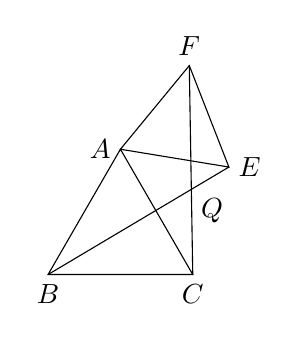
\begin{tikzpicture}[scale=0.45]
                \coordinate[label=left:{$A$}] (A) at (0,0);
                \coordinate[label=below:{$B$}] (B) at (-2.04146,-3.53592);
                \coordinate[label=below:{$C$}] (C) at (2.04146,-3.53592);
                \coordinate[label=right:{$E$}] (E) at (3.06125,-0.50271);
                \coordinate[label=above:{$F$}] (F) at (1.94348,2.36080);
                \coordinate[label=below right:{$Q$}] (Q) at (2.00118,-1.11147);
                \draw (A) -- (B) -- (C) -- cycle;
                \draw (A) -- (E) -- (F) -- cycle;
                \draw (B) -- (E);
                \draw (C) -- (F);
            \end{tikzpicture}
        \end{figure}
        \subquestion \addspace
    \end{subquestions}
    \question %19
    \begin{subquestions}
        \subquestion \addspace
        \subquestion \addspace
    \end{subquestions}
    \question %20
    \begin{subquestions}
        \subquestion \addspace
        \subquestion \addspace
    \end{subquestions}
    \question \qquad \par
    \begin{figure}[!htb]
        \centering
        \subfigure[(1)]{
            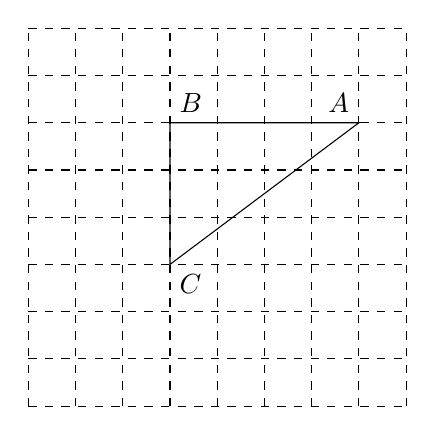
\begin{tikzpicture}[scale=0.6]
                \draw[step=1,dashed] (-3,-3) grid (5,5);
                \coordinate[label=below right:{$C$}] (C) at (0,0);
                \coordinate[label=above left:{$A$}] (A) at (4,3);
                \coordinate[label=above right:{$B$}] (B) at (0,3);
                \draw (A) -- (B) -- (C) -- cycle;
            \end{tikzpicture}}\qquad\qquad
        \subfigure[(2)]{
            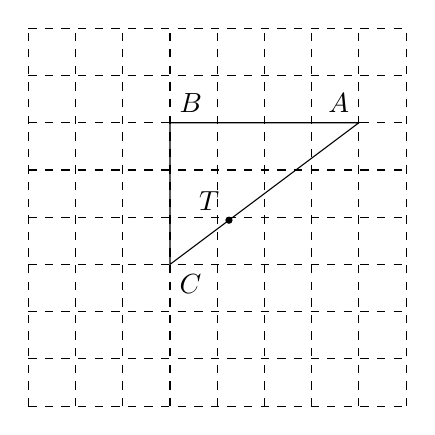
\begin{tikzpicture}[scale=0.6]
                \draw[step=1,dashed] (-3,-3) grid (5,5);
                \coordinate[label=below right:{$C$}] (C) at (0,0);
                \coordinate[label=above left:{$A$}] (A) at (4,3);
                \coordinate[label=above right:{$B$}] (B) at (0,3);
                \coordinate[label=above left:{$T$}] (T) at (1.24848,0.93636);
                \filldraw (T) circle (0.064);
                \draw (A) -- (B) -- (C) -- cycle;
            \end{tikzpicture}
        }
    \end{figure}
    \question %22
    \begin{subquestions}
        \subquestion \addemptyline
        \subquestion %\addspace \addemptyline \addemptyline \addemptyline
        \newpage
        \subquestion \qquad \par
        \begin{figure}[!htb]
            \raggedleft
            \begin{tikzpicture}[>=Stealth,scale=0.5]
                \draw[->] (-7.5,0) -- (4.2,0) node[below] {$x$};
                \draw[->] (0,-1) -- (0,5.5) node[right] {$y$};
                \coordinate[label=below right:{$O$}] (O) at (0,0);
                \draw (0,0) -- (3.5,3.5) -- (4.2,3.5);
                \draw (-7,5) parabola bend (-7,5) (1.5,1.5);
                \filldraw (-7,5) circle (.1);
                \node[below] at (-7,5) {无人机};
                \draw[line width =2pt] (1,1) -- (2,2);
            \end{tikzpicture}
        \end{figure}
    \end{subquestions}
    \addspace \addspace
    \question %23
    \begin{subquestions}
        \subquestion \qquad \par
        \begin{figure}[!htb]
            \raggedleft
            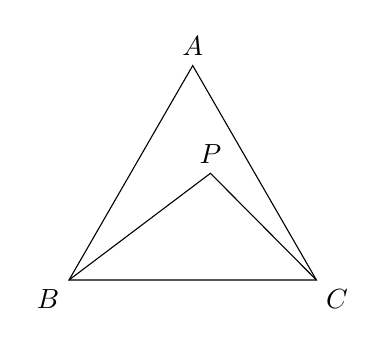
\begin{tikzpicture}[scale=0.45]
                \coordinate[label=above:{$A$}] (A) at (3.49,6.05);
                \coordinate[label=below left:{$B$}] (B) at (0,0);
                \coordinate[label=below right:{$C$}] (C) at (6.98,0);
                \draw (A) -- (B) -- (C) -- cycle;
                \coordinate[label=above:{$P$}] (P) at (3.99,3.01);
                \draw (B) -- (P) -- (C);
            \end{tikzpicture}
        \end{figure}
        \subquestion \qquad \par
        \begin{figure}[!htb]
            \raggedleft
            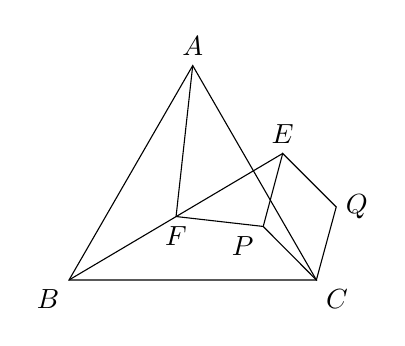
\begin{tikzpicture}[scale=0.45]
            \coordinate[label=above:{$A$}] (A) at (3.49,6.05);
            \coordinate[label=below left:{$B$}] (B) at (0,0);
            \coordinate[label=below right:{$C$}] (C) at (6.98,0);
            \draw (A) -- (B) -- (C) -- cycle;
            \coordinate[label=below left:{$P$}] (P) at (5.48,1.51);
            \coordinate[label=right:{$Q$}] (Q) at (7.54,2.06);
            \coordinate[label=above:{$E$}] (E) at (6.03,3.57);
            \coordinate[label=below:{$F$}] (F) at (3.02,1.79);
            \draw (P) -- (C) -- (Q) -- (E) -- cycle;
            \draw (B) -- (E);
            \draw (A) -- (F) -- (P);
        \end{tikzpicture}
        \par \addspace
        \end{figure}
        \subquestion \newpage
    \end{subquestions}
    \question %24
    \begin{subquestions}
        \subquestion \addemptyline
        \subquestion \qquad \par
        \begin{figure}[!htb]
            \raggedleft
            \begin{tikzpicture}[>=Stealth,scale=0.7]
                \draw[->] (-2,0) -- (5,0) node[below] {$x$};
                \draw[->] (0,-5) -- (0,2) node[right] {$y$};
                \coordinate[label=below right:{$O$}] (O) at (0,0);
                \draw (-1.24,1) parabola bend (1,-4) (3.24,1);
                \coordinate[label=below left:{$A$}] (A) at (-1,0);
                \coordinate[label=below right:{$B$}] (B) at (3,0);
                \coordinate[label=left:{$C$}] (C) at (0,-3);
                \draw (B) -- (C);
                \draw (0.8,-5) -- (0.8,2);
                \coordinate[label=left:{$E$}] (E) at (0.8,-2.2);
                \coordinate[label=left:{$F$}] (F) at (0.8,-3.96);
                \draw (1.8,-5) -- (1.8,2);
                \coordinate[label=left:{$M$}] (M) at (1.8,-1.2);
                \coordinate[label=left:{$N$}] (N) at (1.8,-3.36);
            \end{tikzpicture}
        \end{figure}
        \addspace
        \subquestion \qquad \par
        \begin{figure}[!htb]
            \raggedleft
            \begin{tikzpicture}[>=Stealth,scale=0.7]
                \draw[->] (-2,0) -- (5,0) node[below] {$x$};
                \draw[->] (0,-5) -- (0,2) node[right] {$y$};
                \coordinate[label=below right:{$O$}] (O) at (0,0);
                \draw (-1.24,1) parabola bend (1,-4) (3.24,1);
                \coordinate[label=below left:{$A$}] (A) at (-1,0);
                \coordinate[label=below right:{$B$}] (B) at (3,0);
                \coordinate[label=below:{$D$}] (D) at (1,-4);
                \draw (-1.52,-1.22) -- (4.46,-2.54);
                \coordinate[label=below:{$P$}] (P) at (-0.60,-1.43);
                \coordinate[label=below right:{$Q$}] (Q) at (2.38,-2.08);
                \draw (-1.51,-1.79) -- (4.80,0.71);
                \draw (0.54,-4.64) -- (4.76,1.20);
                \coordinate[label=below right:{$T$}] (T) at (4.25,0.49);
                \draw (A) -- (T);
            \end{tikzpicture}
        \end{figure}
    \end{subquestions}
\end{questions}
\end{document}